\documentclass[11pt, a4paper]{article}
%\usepackage{proj1}
\usepackage{natbib}
\usepackage{fancyhdr}  
\usepackage{subcaption}
\usepackage{caption}
\usepackage{graphicx}
\linespread{1.25} 
\setlength{\parindent}{0cm}
\graphicspath{{Images/}}
\usepackage{hyperref}
\usepackage{amsmath}
\usepackage{amsfonts}
\usepackage{amssymb}
\usepackage{amsthm}
\usepackage{mathtools}
\usepackage{commath}

%\usepackage[sc,osf]{mathpazo}
\usepackage{subcaption}
\usepackage[a4paper, top=1in, left=1.0in, right=1.0in, bottom=1in, includehead, includefoot]{geometry} %Usually have top as 1in

\usepackage{listings}
\usepackage{color} %red, green, blue, yellow, cyan, magenta, black, white
\definecolor{mygreen}{RGB}{28,172,0} % color values Red, Green, Blue
\definecolor{mylilas}{RGB}{170,55,241}


\hypersetup{colorlinks,linkcolor={black},citecolor={blue},urlcolor={black}}
\usepackage{color}
\urlstyle{same}


\theoremstyle{definition}
\newtheorem{definition}{Definition}[section]

\title{Exact Solutions for the Full Problem \\with Force Control and with Flow Control}
\date{}
\newcommand{\Sta}{\rho}
\newcommand{\Adj}{p}
\newcommand{\Con}{u}

\pagenumbering{gobble}
\begin{document}



\section*{Linear time exact solution trials}

\subsection*{Perturbation Functions Considered}
The one from last week:
\begin{align*}
f(t) = \frac{e^{-1/t}}{e^{-1/t} + e^{-1/(1-t)}}.
\end{align*}
An new perturbation is given by:
\begin{align*}
g(t) = \frac{e^{-a/(t-t0)}}{e^{-a/(t-t0)}+ e^{-a/(1-t-t0)}} \times \frac{e^{a/(t-t0)}}{e^{a/(t-t0)}+ e^{a/(1-t-t0)}},
\end{align*}
where $a=0.7$ (mostly) and $t0 = -0.01$. The translation by $t0$ is due to the fact that otherwise you'd get NANs for $t=0$. The factor $a$ is flattening or sharpening the peak.\\
\begin{figure}[h]
	\includegraphics[scale=0.3]{Pertfun2.jpg}
	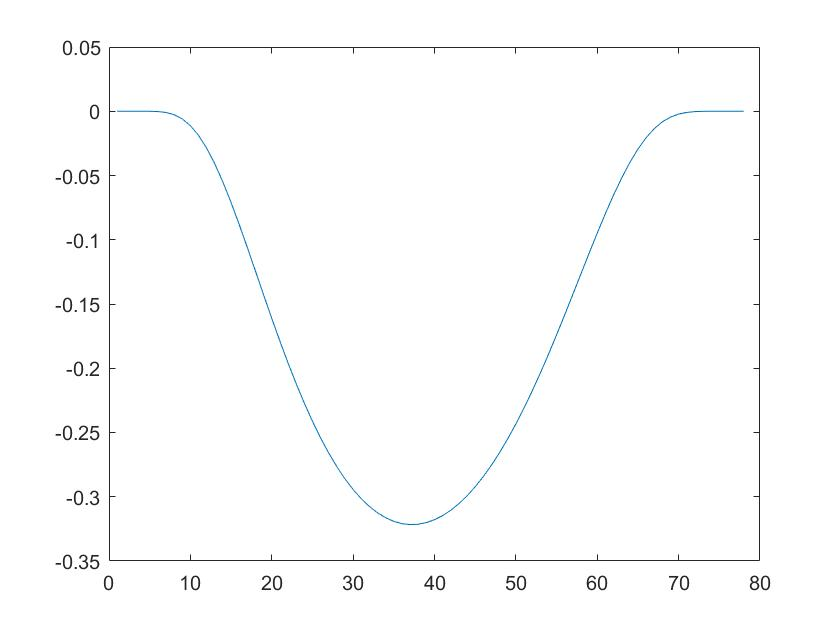
\includegraphics[scale=0.3]{wPert3.jpg}
	\caption{Perturbation $g(t)$ (left), $w$ perturbed by $0.1g(t)$ (right).}
\end{figure}

Finally, we consider a similar perturbation in space. 
\begin{align*}
h(x) = \frac{e^{-a/(1+x-x0)}}{e^{-a/(1+x-x0)}+ e^{-a/(1-x-x0)}} \times \frac{e^{a/(1+x-x0)}}{e^{a/(1+x-x0)}+ e^{a/(1-x-x0)}},
\end{align*}
where an extra factor of $1$ is added to the denominator to account for the space interval being $[-1,1]$ and not $[0,1]$. The factor $a$ is the same as above and $x0 = t0$. The function and the effect on $w$ can be seen in Figure \ref{ypert1}.
\begin{figure}[h]
	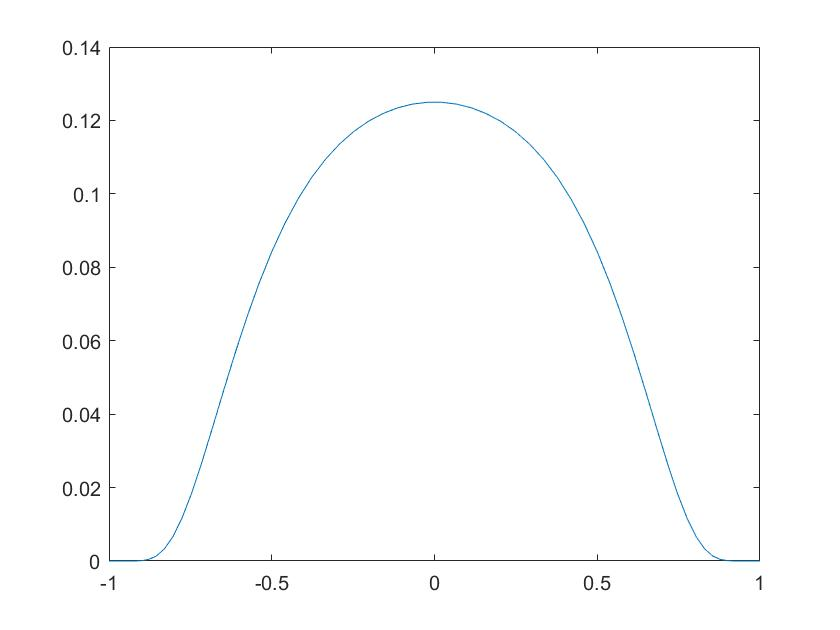
\includegraphics[scale=0.3]{yPert1.jpg}
	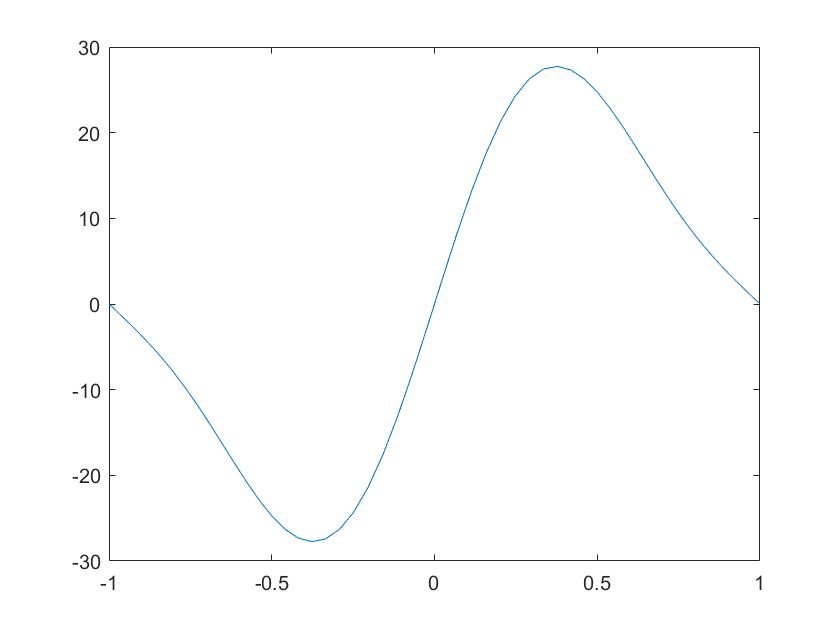
\includegraphics[scale=0.3]{wperty1.jpg}
	\caption{Perturbation $h(x)$ (left), $w$ perturbed by $h(x)$ (right).}
	\label{ypert1}
\end{figure}



\subsection*{Kalise}
\subsubsection*{Mixed3}
We are using the exact solution 'Mixed3' (second version of the Mixed BC exact solutions) with Dirichlet and Neumann BCs. All errors are measured in L2Linf, tolerances and $n,N$ as above.
In the Dirichlet Case both $\beta = 10^{-1}$ ($\lambda =0.1$) and $\beta = 10^{-3}$ ($\lambda =10$) converged. The perturbation was $10g(t)$ with $a=0.7$, see Figure \ref{Figlint1} and \ref{Figlint2}.
For $\beta=10^{-1}$ the initial exact error was $w_{errI}= 0.0324$, $p_{errI} = 0.0557$ and $\rho_{errI}= 0.0421$. Then after $1157$ iterations it converged to $w_{err}= 2.2602 \times  10^{-7}$, $p_{err} = 4.2460 \times 10^{-7}$ and $\rho_{err} = 31175 \times 10^{-7}$. The errors for $\beta = 10^{-3}$ are similar.\\
The results for the Neumann case are very similar. The algorithm converges for both $\beta$ values. 
For $\beta = 10^{-1}$ the initial exact errors are $w_{ErrI}=0.0309$, $p_{errI} = 0.0755$ and $\rho_{ErrI}= 0.0466$. Then in $1175$ Iterations, this converges to $w_{err}= 2.1936 \times 10^{-7}$, $p_{Err}=6.5744 \times 10^{-7}$ and $\rho_{err} = 3.4265 \times 10^{-7}$. The results for $\beta = 10^{-3}$ are again similar.\\
\begin{figure}[h]
	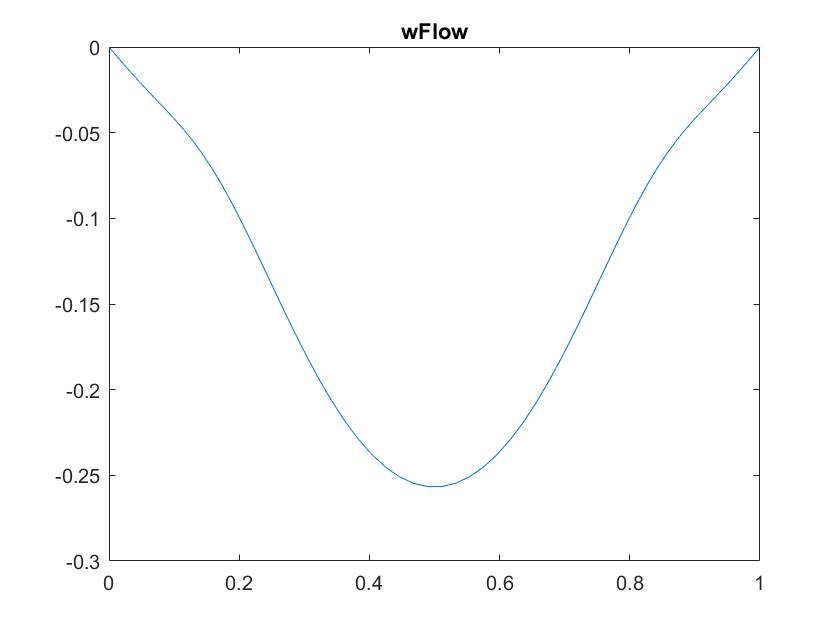
\includegraphics[scale=0.3]{wFlint3.jpg}
	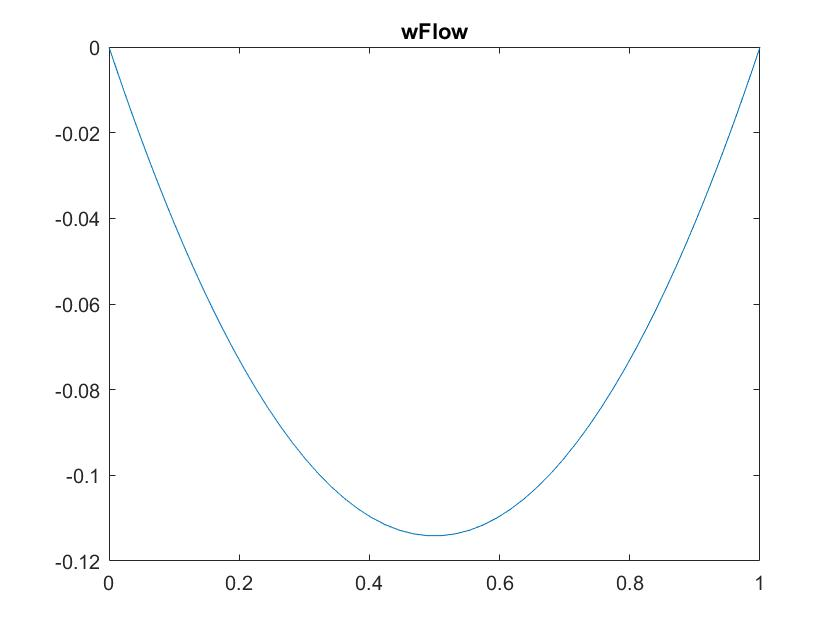
\includegraphics[scale=0.3]{wFlint4.jpg}
	\caption{Perturbed $w$ and exact $w$.}
	\label{Figlint1}
\end{figure}
\begin{figure}[h]
	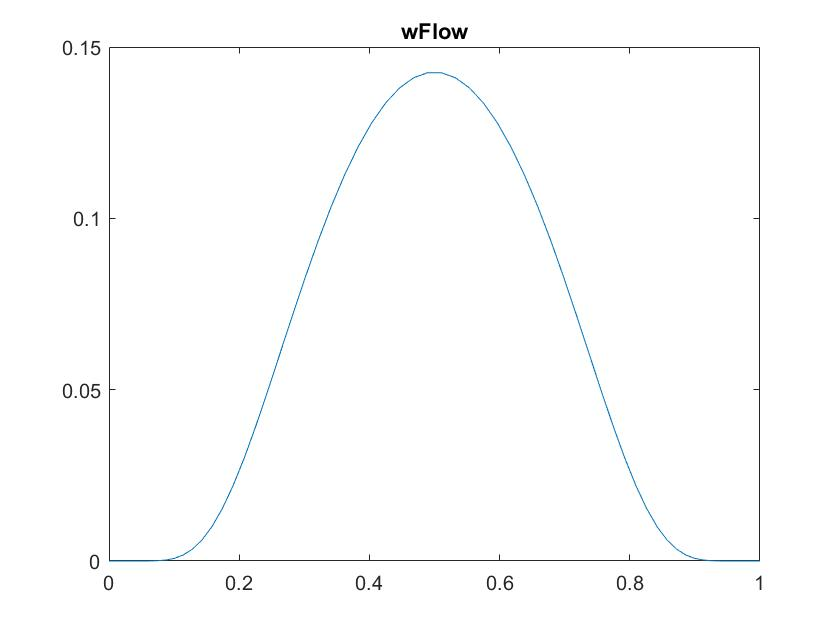
\includegraphics[scale=0.2]{wFlint1.jpg}
	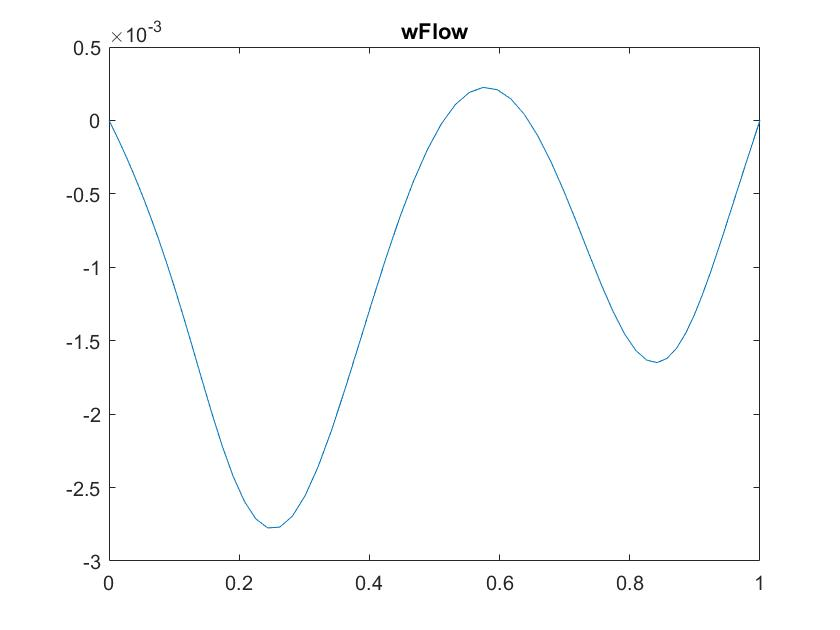
\includegraphics[scale=0.2]{wFlint2.jpg}
	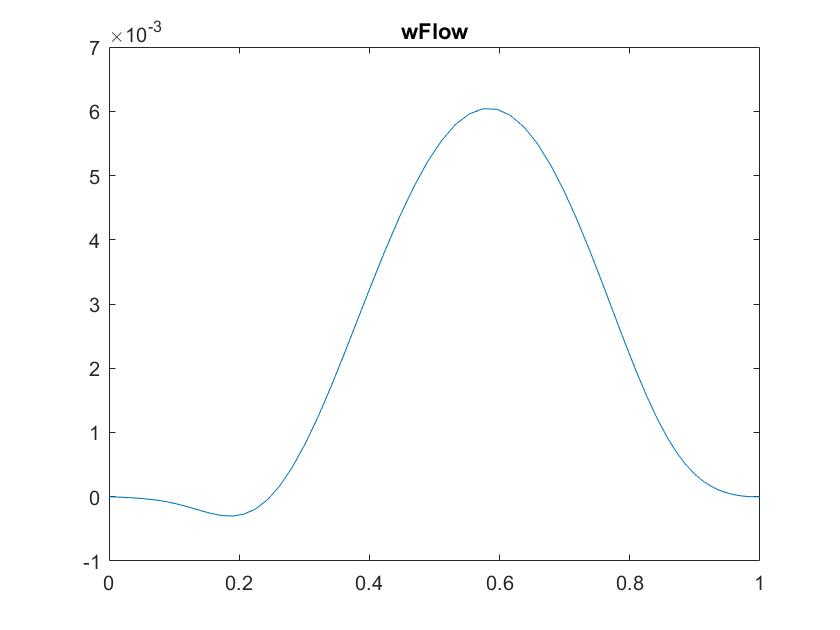
\includegraphics[scale=0.2]{wFlint5.jpg}
	\caption{Perturbed $w$ Error (first - left) (second: Dirichlet - Mid, Neumann - right).}
	\label{Figlint2}
\end{figure}
\subsubsection*{Neumannplus2 linear time, trig space}
Now, investigating Neumann (plus 2) with linear time terms (i.e. exact solution with trig functions in space, and linear time) gives the following: With $\beta=10^{-1}$ the initial errors are $w_{errI} = 0.2353$, $p_{errI} = 0.8576$ and $\rho_{errI}=0.3192$. This converges in $1167$ Iterations to $w_{err}=6.9449 \times 10^{-7}$, $p_{err}= 8.3209 \times 10^{-6}$ and $\rho_{err}= 2.1389 \times 10^{-6}$. The results are very similar for $\beta=10^{-3}$ and can be seen in Figure \ref{Figlint3}. The perturbation in $w$ can be seen in Figure \ref{Figlint3a}. Note this also converges to  a tolerance of $10^{-6}$ instead of $10^{-5}$.\\
\begin{figure}[h]
	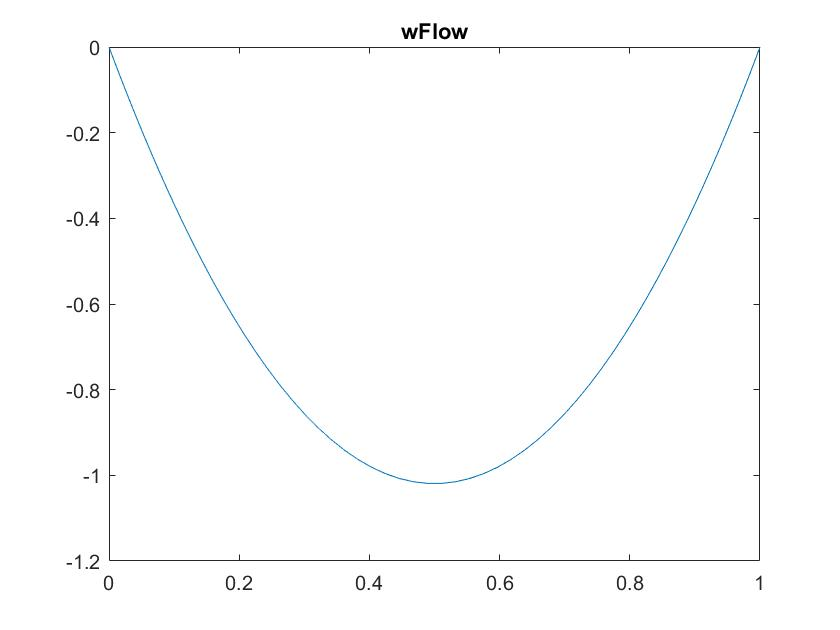
\includegraphics[scale=0.3]{linNwexact1.jpg}
	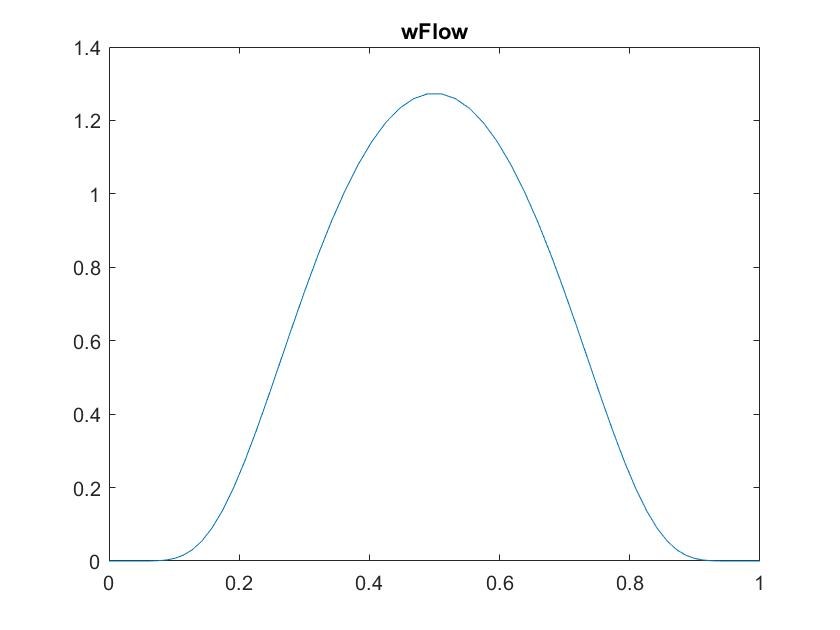
\includegraphics[scale=0.3]{linNwerr1.jpg}
	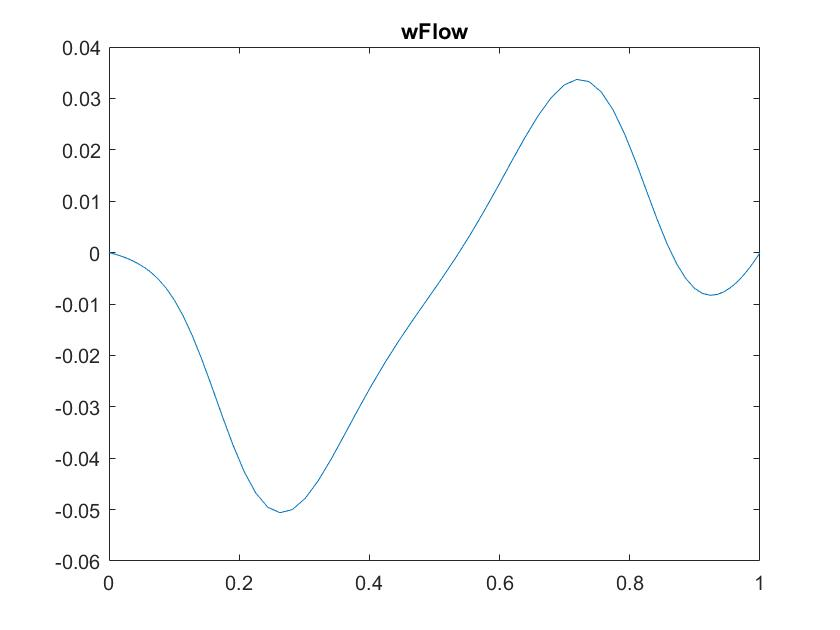
\includegraphics[scale=0.3]{linNwerr2.jpg}
	\caption{This is $w$ exact (left), $w$ first error (mid) and second error (right). Here with $\beta =10^{-3}$ and perturbation $10g(t)$.}
	\label{Figlint3a}
\end{figure}

\begin{figure}[h]
	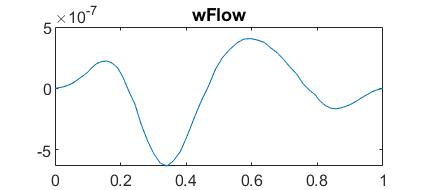
\includegraphics[scale=0.35]{linNfin1.jpg}
	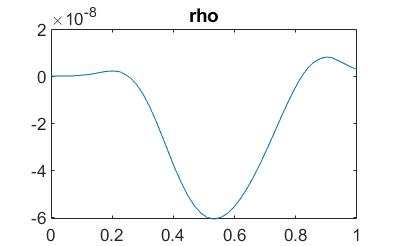
\includegraphics[scale=0.35]{linNfin2.jpg}
	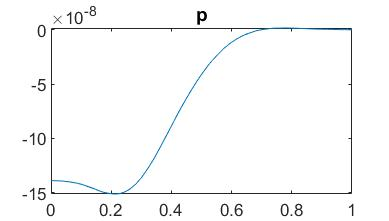
\includegraphics[scale=0.35]{linNfin3.jpg}
	\caption{Final error in variables when Neumann with linear time converged. Here with $\beta =10^{-3}$ and perturbation $10g(t)$.}
	\label{Figlint3}
\end{figure}

\subsubsection*{Dirichlet linear time, trig space (1)}

Looking at Dirichlet Exact solutions with linear time terms (i.e. trig in space, linear in time), this also converges for the two $\beta$ values. Accidentally the tolerance was set to $10^{-6}$ which converged as well ($\beta = 10^{-1}$. The perturbations in $w$ can be seen in Figure \ref{Figlint4a}.
The results are $w_{err} = 8.6507 \times 10^{-7}$, $p_{err} = 2.9450 \times 10^{-7}$ and $\rho_{Err}= 10^{-7}$. \\
Considering $\beta+10^{-3}$ seems to be a bit more difficult, simply because the scaling makes the perturbation much larger for this case. Therefore, different perturbations have to be tried, to see which one perturbs $w$ a reasonable amount. It seems like even very small perturbations cannot reach convergence. This is most likely due to the fact that the Dirichlet exact solution for $w$ scales like $1/\beta$ (to be consistent with the original exact solutions). This is discussed next.\\
\begin{figure}[h]
	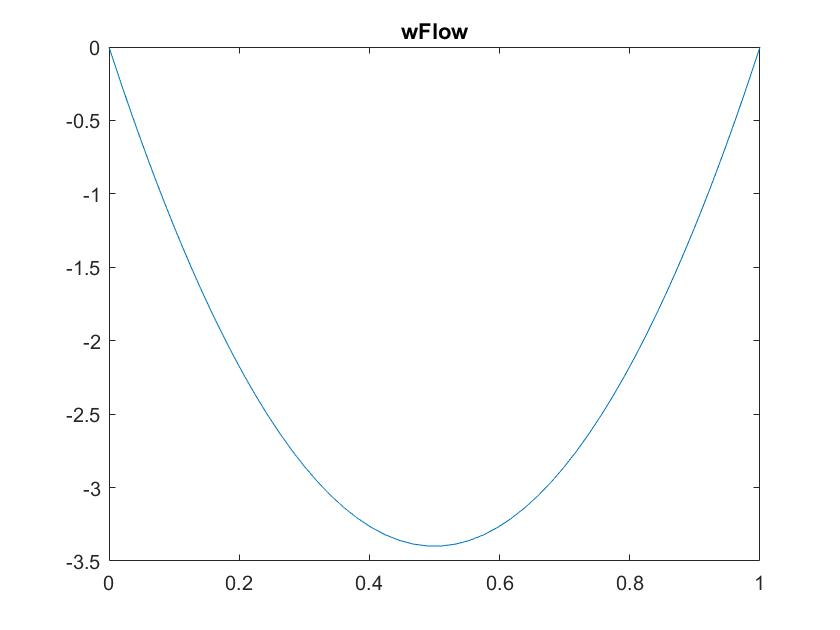
\includegraphics[scale=0.3]{linDwexact1.jpg}
	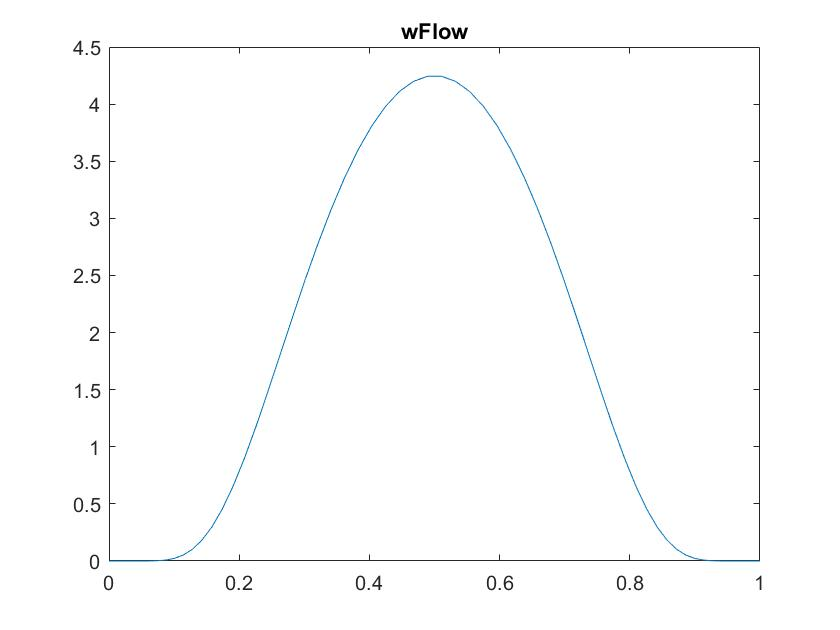
\includegraphics[scale=0.3]{linDwerr1.jpg}
	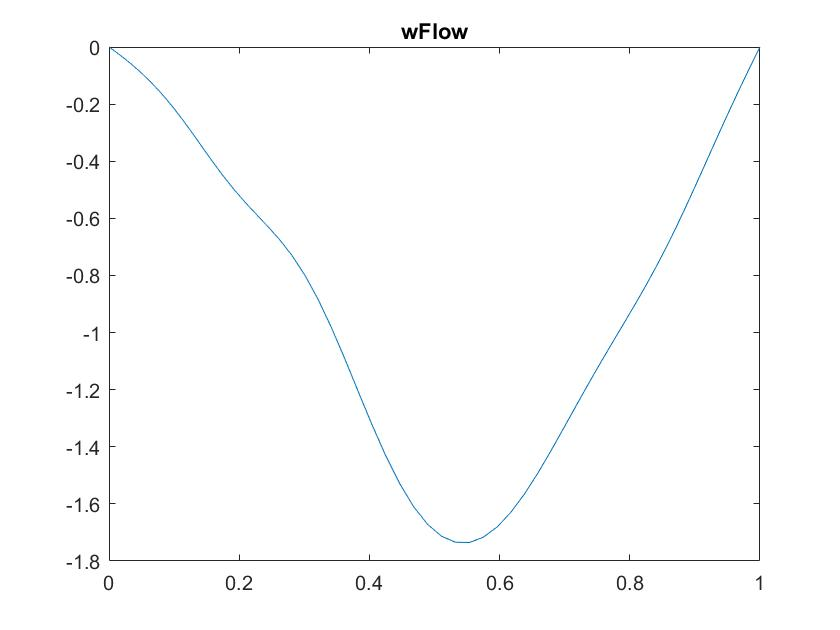
\includegraphics[scale=0.3]{linDwerr2.jpg}
	\caption{This is $w$ exact (left), $w$ first error (mid) and second error (right). Here with $\beta =10^{-1}$ and perturbation $10g(t)$.}
	\label{Figlint4a}
\end{figure}
\subsubsection*{Dirichlet linear time, trig space (2)}
Scaling $\rho{Exact}$ and $p_{Exact}$ with $\beta^{1/2}$ makes $w_{Exact}$ independent of $\beta$. Trying again $10*g(t)$ and it can be observed that the magnitude of perturbation looks more reasonable now, see Figures \ref{Figlint4c} and \ref{Figlint4d}.
With $\beta = 10^{-3}$ and $\lambda =10$, we get final errors at Iteration $1132$ of $w_{err} = 4.4521 \times 10^{-7}$, $p_{err} = 5.9025 \times 10^{-7}$ and $\rho_{err} = 4.8031 \times 10^{-7}$, see Figure \ref{Figlint4b}. The initial errors for this were $w_{errI} = 0.1037$, $p_{errI} = 0.0885$ and $\rho_{errI} = 0.0737$. The results for $\beta = 10^{-1}$ look basically the same.

\begin{figure}[h]
	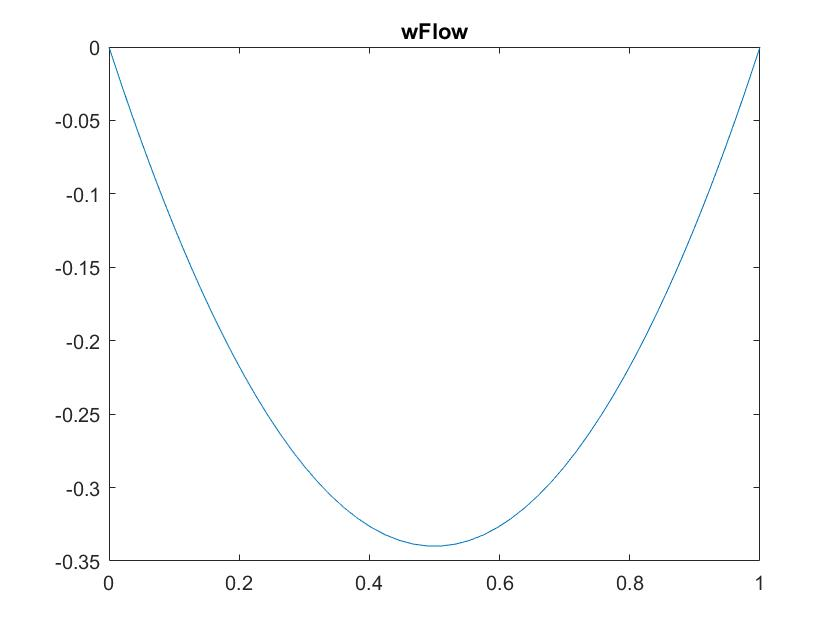
\includegraphics[scale=0.3]{KalDneww3.jpg}
	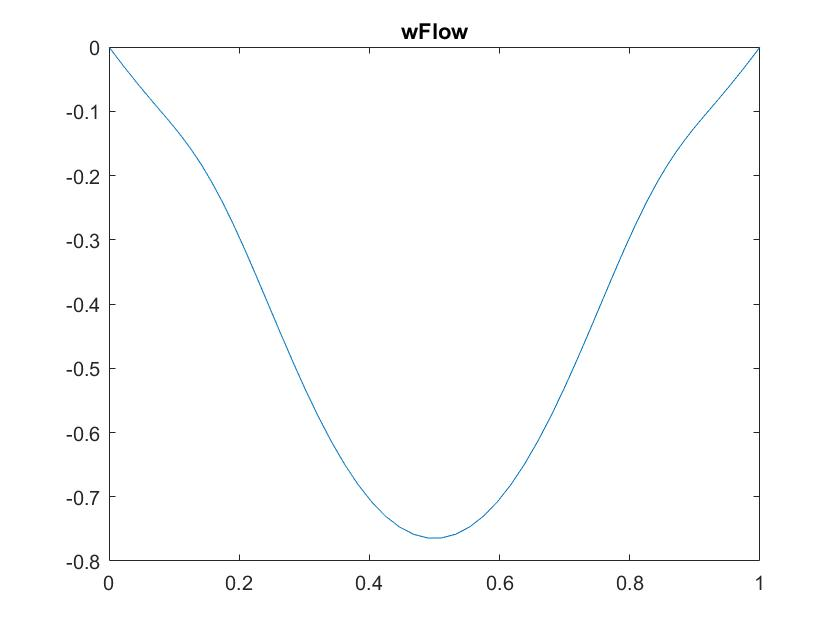
\includegraphics[scale=0.3]{KalDneww4.jpg}
	\caption{Exact $w$ and perturbed $w$. Here with $\beta =10^{-3}$ and perturbation $10g(t)$.}
	\label{Figlint4c}
\end{figure}
\begin{figure}[h]
	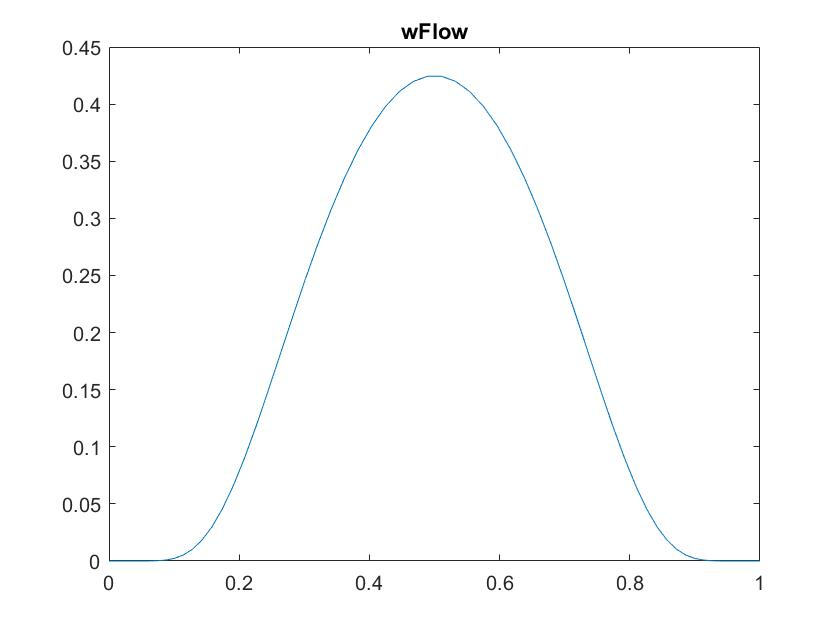
\includegraphics[scale=0.3]{KalDneww1.jpg}
	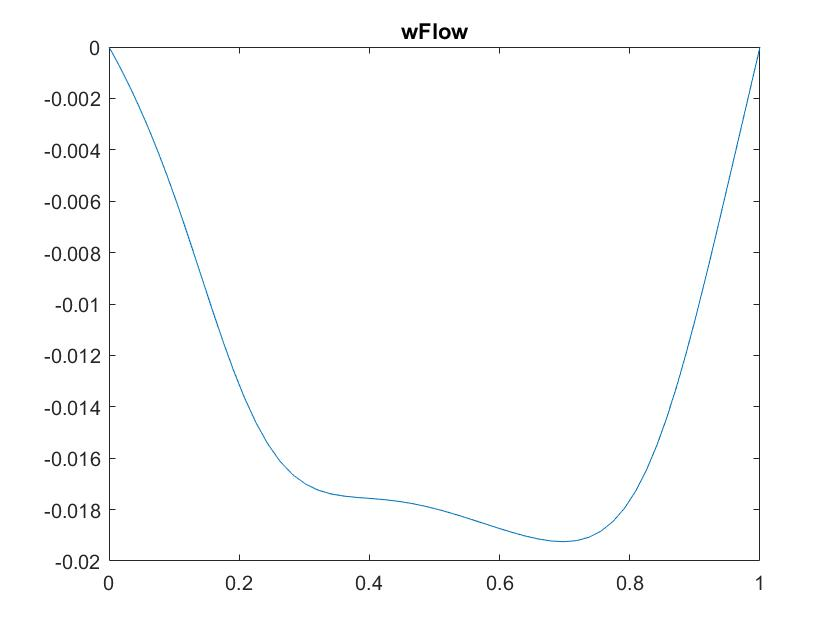
\includegraphics[scale=0.3]{KalDneww2.jpg}
	\caption{$w$ error 1 (left) and 2 (right). Here with $\beta =10^{-3}$ and perturbation $10g(t)$.}
	\label{Figlint4d}
\end{figure}



\begin{figure}[h]
	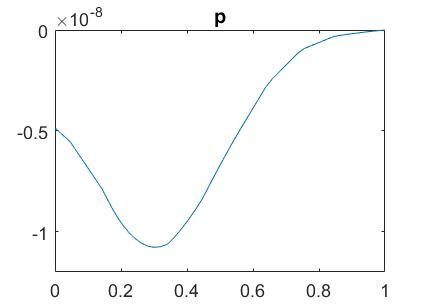
\includegraphics[scale=0.3]{KalDnew1.jpg}
	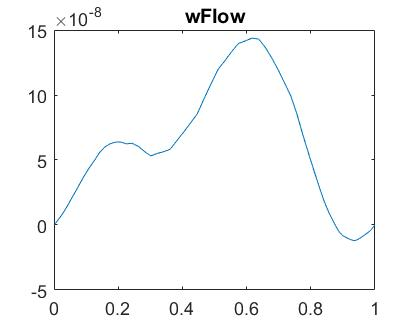
\includegraphics[scale=0.3]{KalDnew2.jpg}
	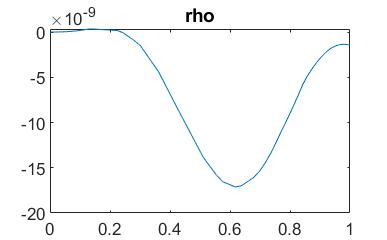
\includegraphics[scale=0.3]{KalDnew3.jpg}
	\caption{Exact final errors. Here with $\beta =10^{-3}$ and perturbation $10g(t)$.}
	\label{Figlint4b}
\end{figure}


\subsection*{Multiple Shooting}
\subsubsection*{Mixed3}
Using 'Mixed3' again with Dirichlet BCs, and the perturbation $10g(t)$,with $\beta=10^{-1}$ and measured in L2Linf norm, Multiple Shooting converges within $724$ Iterations. The exact errors are then $\rho_{err} = 0.00000791$ and $p_{err}=0.00015429$, see Figure \ref{Figlint5}. The initial errors were $cons_{err} = 0.02820414$, $\rho_{ErrI} = 0.03215880$ and $p_{err} = 0.01302147$. \\

\begin{figure}[h]
	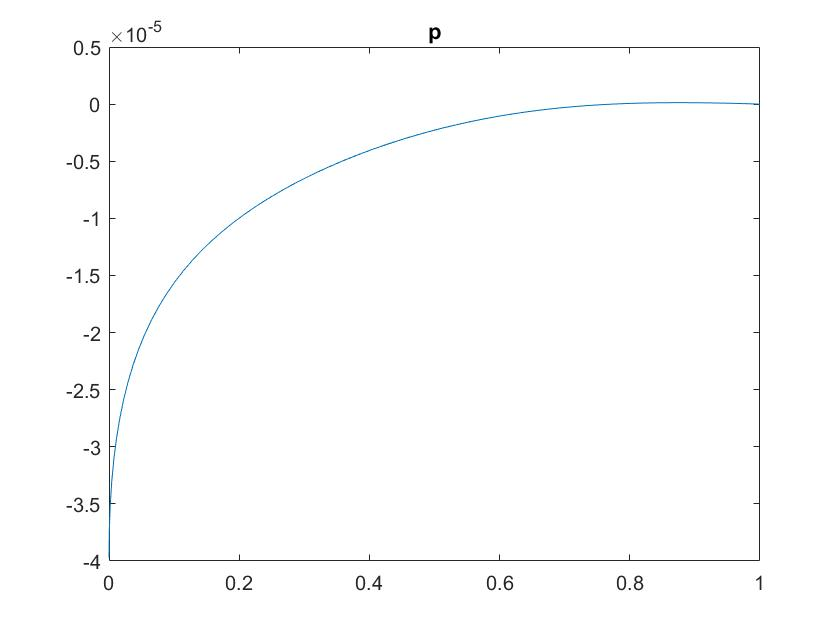
\includegraphics[scale=0.3]{MultMD1.jpg}
	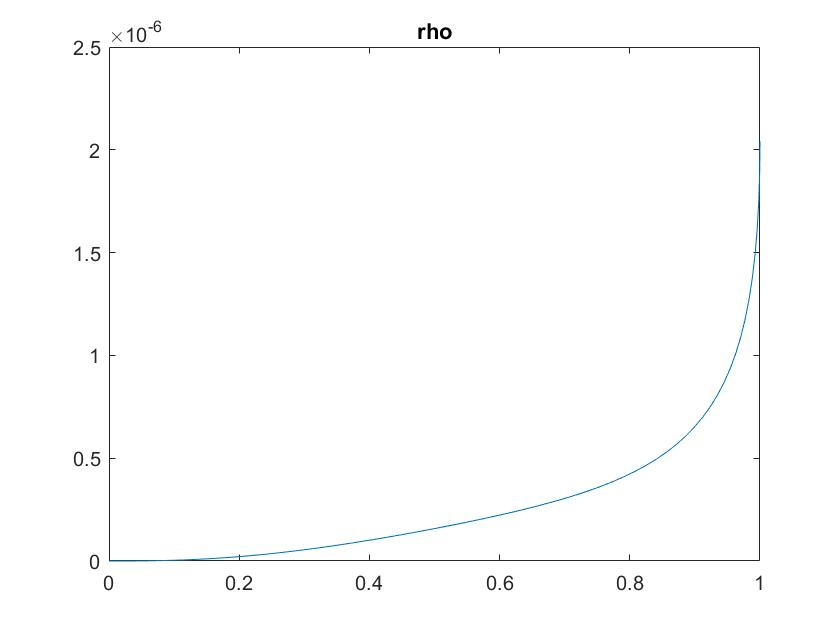
\includegraphics[scale=0.3]{MultMD2.jpg}
	\caption{Final exact error in $\rho$ and $p$. Here with $\beta =10^{-1}$ and perturbation $10g(t)$.}
	\label{Figlint5}
\end{figure}
The algorithm also converges for Neumann BCs using $10g(t)$. The initial error is $0.01835403$, $\rho_{errI} = 0.03490495$ and $p_{errI}= 0.00321550$. Then, after $481$ iterations, the algorithm converges and gives $\rho_{err} = 0.00000738$ and $p_{err}= 0.00009099$.

\subsubsection*{Neumann plus2 linear t}

Using $10g(t)$ and $\beta=10^{-1}$, $\lambda =0.1$ converges. The initial errors were $0.19989140$, $\rho_{errI} = 0.25206626$ and $p_{errI}= 0.09993510$. It converges in $982$ Iterations to $\rho_{err} = 0.00000003$ and $p_{err} = 0.00001598$, see Figure \ref{Figlint6}. With $\beta=10^{-3}$ the result is basically the same, only takes double the iterations at the same $\lambda$. 



\begin{figure}[h]
	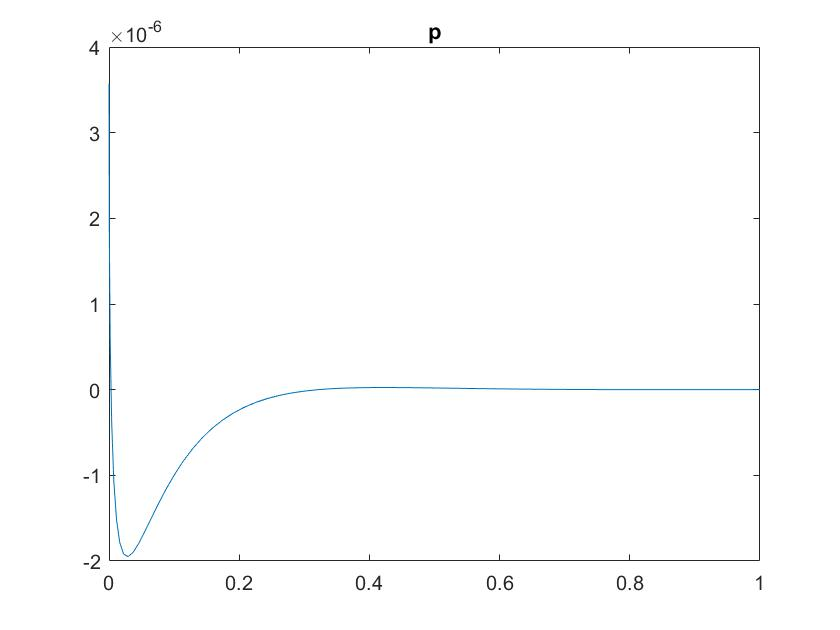
\includegraphics[scale=0.3]{MultNp21.jpg}
	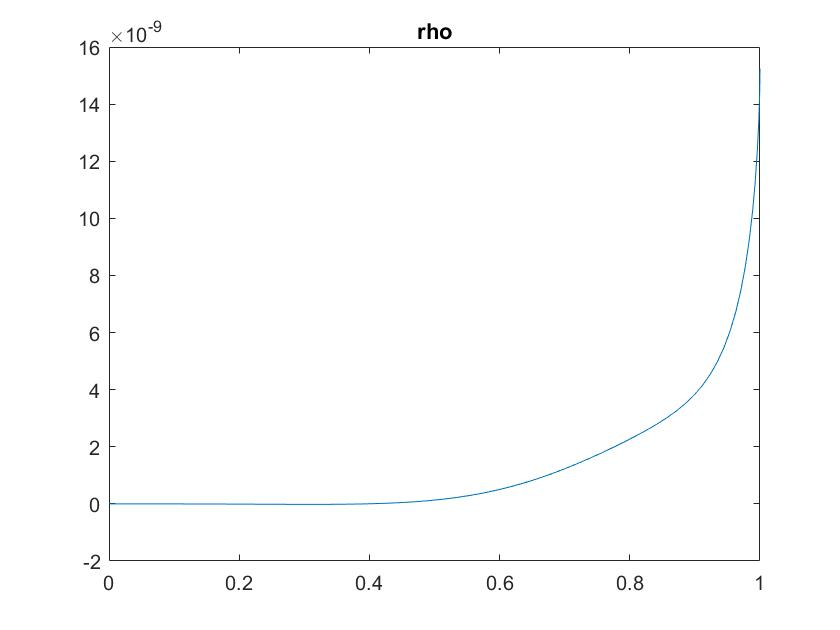
\includegraphics[scale=0.3]{MultNp22.jpg}
	\caption{Final exact error in $\rho$ and $p$. Here with $\beta =10^{-1}$ and perturbation $10g(t)$.}
	\label{Figlint6}
\end{figure}


\subsubsection*{Dirichlet linear t (2)}
This also converges for $10 g(t)$, $\beta =10^{-1}$ and $\lambda = 10^{-1}$.
The initial errors are $conc_{err} = 0.08618302$, $\rho_{errI} = 0.06506113$ and $p_{errI}=0.06437616$. After $948$ Iterations it converges and the errors are $\rho_{err} = 0.00000700$ and $p_{err} = 0.00005981$. This is similar for $\beta = 10^{-3}$.

\subsection*{Trying original perturbation $f(t)$ - Kalise}
Just a check that the original perturbation $f(t)$ also works on this version of the Neumann problem (as it had with the exponential exact solutions). Furthermore, does the Dirichlet problem now converge with this?
Yes to both. Tried Neumann with $\beta = 10^{-3}$ and it converges in $1078$ Iterations from O$(10^{-1})$ to O$(10^{-7})$.
Similarly, chose Dirichlet with $\beta = 10^{-1}$ and got similar convergence results for this.



\subsection*{Trying $g(t)h(x)$ perturbation}
\subsubsection*{Kalise}
Starting with Kalise and Neumann(plus2) Flow control, we choose the perturbation $100g(t)h(x)$, see first section in document. The effect of $w$ can be seen in Figure \ref{Figgh1}.
Choosing $\beta = 10^{-1}$, $\lambda=0.1$, the initial error is $w_{errI}= 0.2627$, $p_{ErrI}= 0.7837$ and $\rho_{errI}=0.3350$, with consistency error of $w_{cons}= 0.6782$. After $1142$ Iterations this converges to $w_{err} = 7.1695 \times10^{-7}$, $p_{err} = 8.3103 \times 10^{-6}$ and $\rho_{err} = 2.2422 \times 10^{-6}$. Choosing $\beta =10^{-3}$ works as well.
THe dirichlet case with $\beta = 10^{-1}$ converges as well in $1124$ itrations and the solutions are of order $10^{-6}/10^{-7}$.
\begin{figure}[h]
	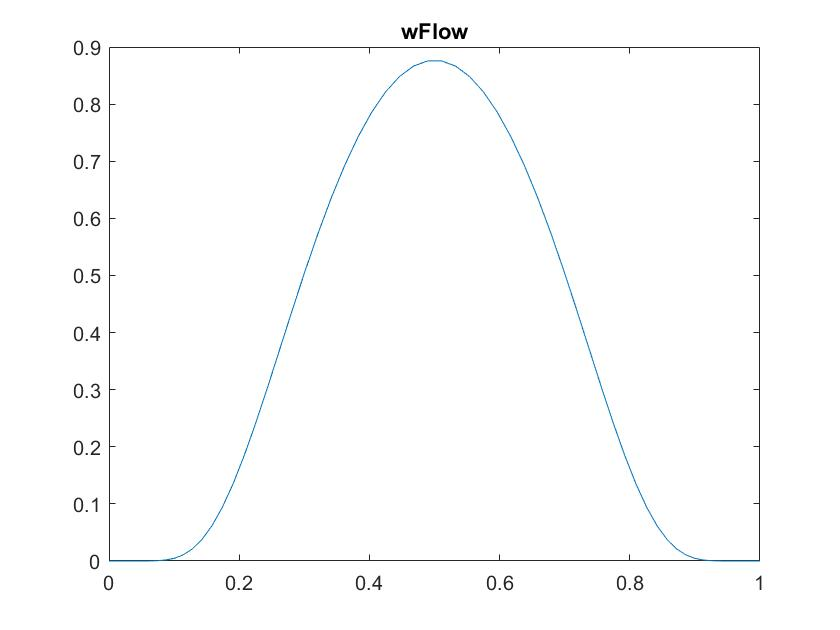
\includegraphics[scale=0.3]{wPertyt1.jpg}
	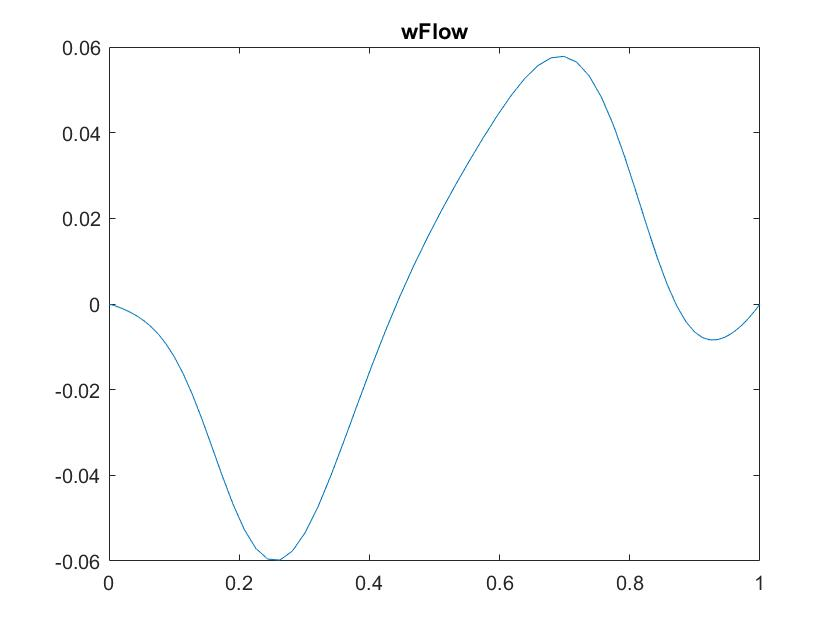
\includegraphics[scale=0.3]{wPertyt2.jpg}
	\caption{First and second error in $w$. Here with $\beta =10^{-1}$ and perturbation $10g(t)h(x)$.}
	\label{Figgh1}
\end{figure}

Trying a larger perturbation $100g(t)h(x)$ for the Neumann case with $\beta =10^{-1}$ gives the two initial errors in $w$ as seen in Figure \ref{Figgh2}. The initial errors are $w_{errI}=0.9313$, $p_{errI}=2.3058$ and $\rho_{ErrI}=1.2690$. After $1355$ Iterations this converges to $w_{err}= 7.0739 \times 10^{-7}$, $p_{err}=8.3938 \times 10^{-6}$ and $\rho_{err} = 2.2085 \times 10^{-6}$. 

\begin{figure}[h]
	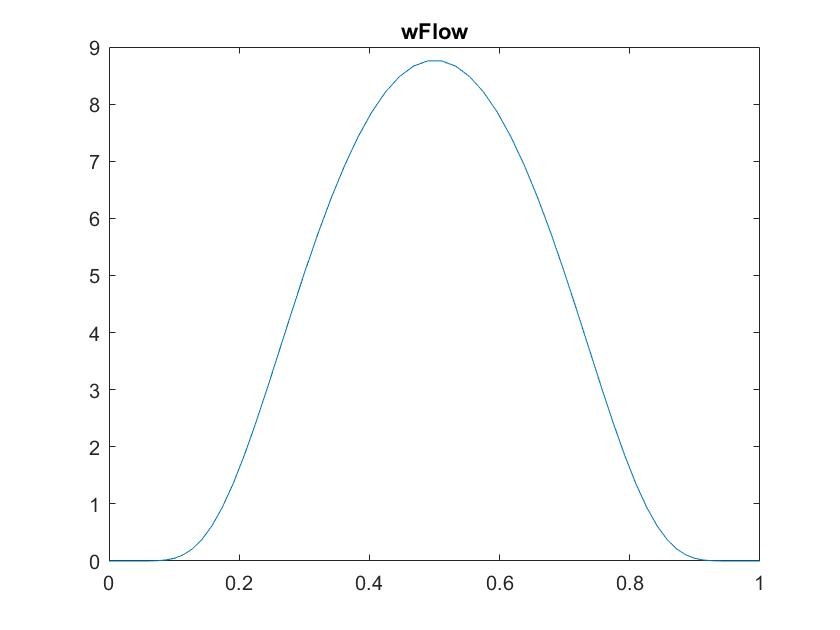
\includegraphics[scale=0.3]{wPertyt3.jpg}
	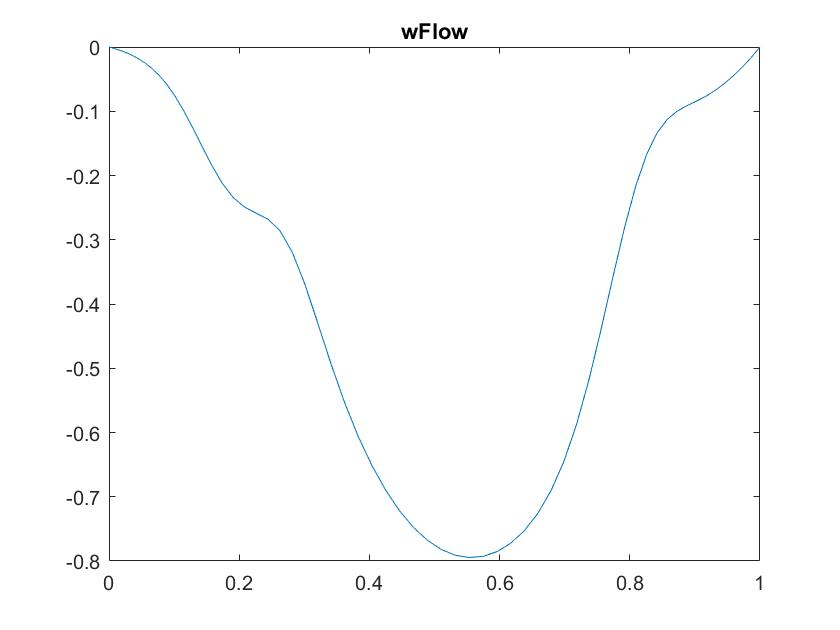
\includegraphics[scale=0.3]{wPertyt4.jpg}
	\caption{First and second error in $w$. Here with $\beta =10^{-1}$ and perturbation $100g(t)h(x)$.}
	\label{Figgh2}
\end{figure}
This larger perturbation also converges for Dirichlet with $\beta = 10^{-1}$, however, the perturbations seems a bit smaller, see Figure \ref*{Figgh3}
Initial errors are $w_{errI}=0.6337$, $p_{errI}=0.5188$ and $\rho_{errI}= 0.5428$.
Then after $1345$ Iterations, the errors are $w_{err}=4.4080 \times 10^{-7}$, $p_{err}=5.4380 \times 10^{-7}$ and $\rho_{err}=5.2775 \times 10^{-7}$. Note that Figure \ref{Figgh3} shows the perturbations in time, while Figure \ref{Figgh4} shows the perturbations in space.

\begin{figure}[h]
	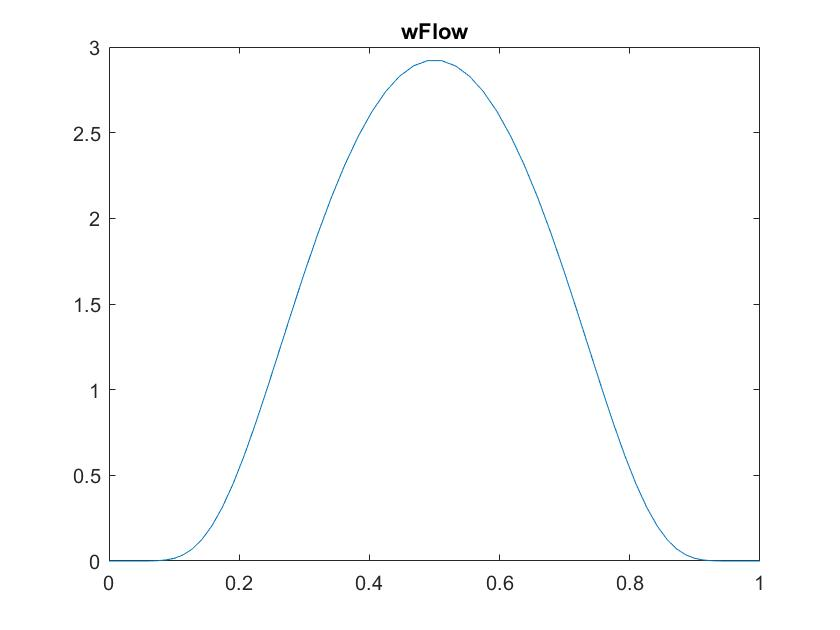
\includegraphics[scale=0.3]{wPertyt5.jpg}
	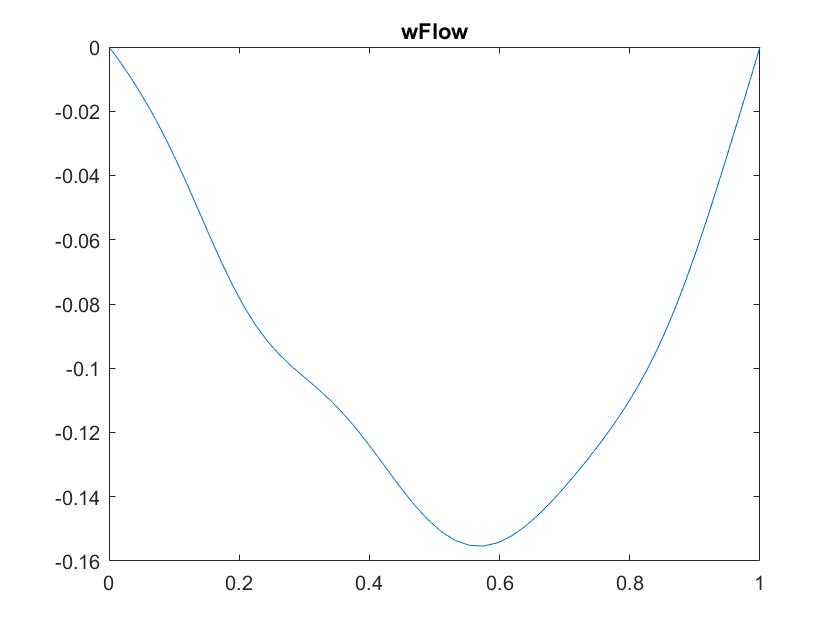
\includegraphics[scale=0.3]{wPertyt6.jpg}
	\caption{First and second error in $w$. Here with $\beta =10^{-1}$ and perturbation $100g(t)h(x)$.}
	\label{Figgh3}
\end{figure}
\begin{figure}[h]
	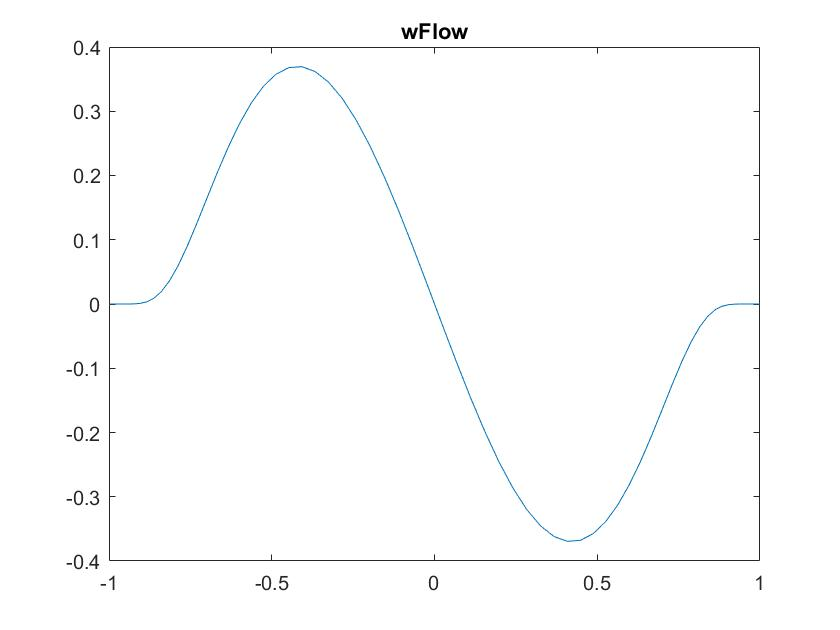
\includegraphics[scale=0.3]{wPertyt7.jpg}
	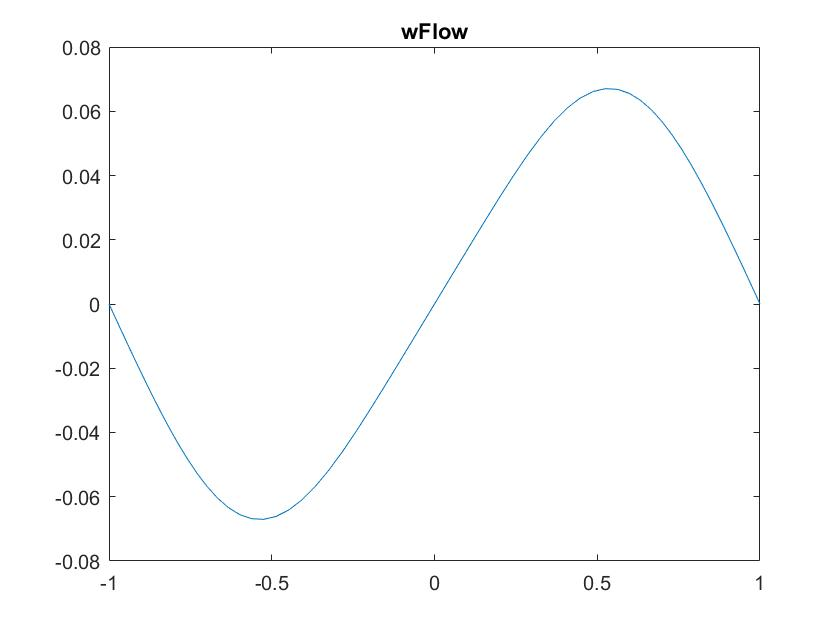
\includegraphics[scale=0.3]{wPertyt8.jpg}
	\caption{First and second error in $w$ in space. Here with $\beta =10^{-1}$ and perturbation $100g(t)h(x)$.}
	\label{Figgh4}
\end{figure}


\subsubsection*{Multiple Shooting}


Both Dirichlet and Neumann converge for $\beta = 10^{-1}$ and $100g(t)h(x)$. Need between $900$ and $1000$ Iterations. 
 








\end{document}